% вторая часть

\section{Анализ существующих продуктов со схожим функционалом}
В ходе подготовки к процессу разработки приложения был проведен анализ магазина мобильных приложений (Google Play) для проверки на наличие аналогичных разработок или разработок схожей тематики.

По результатам анализа оказалось, что такой реализации преобразования фотографий в 3D нет. Однако в этой категории есть ряд похожих разработок, направленных на оживление «плоских» снимков. 

\subsection{Make It 3d Free}

Приложение, позволяющее создать красно-синий анаглиф либо на основе снимка из фотогалереи смартфона, либо сделав снимок прямо из приложения. Стоит заметить, что анаглиф создается на основе двух снимков:  левого и правого, - что само по себе является естественным способом создание объемного изображения, а значит должно гарантировать получение качественного 3D-изображения. После прикрепления двух изображений доступны возможности изменения стереоэффекта: смещение или поворот одного из изображений по или против часовой стрелки. Есть возможность сохранения результата в виде широкого изображения с разделением зон на правый и левый глаз, что может пригодиться для просмотра снимка в устройстве виртуальной реальности (например, в кардборде). По завершении работы, фото экспортируется в галерею и открывается стандартном просмотрщике изображений девайса. (рисунок ~\ref{fig:MakeIt})

\begin{figure}[H]
	\centering
	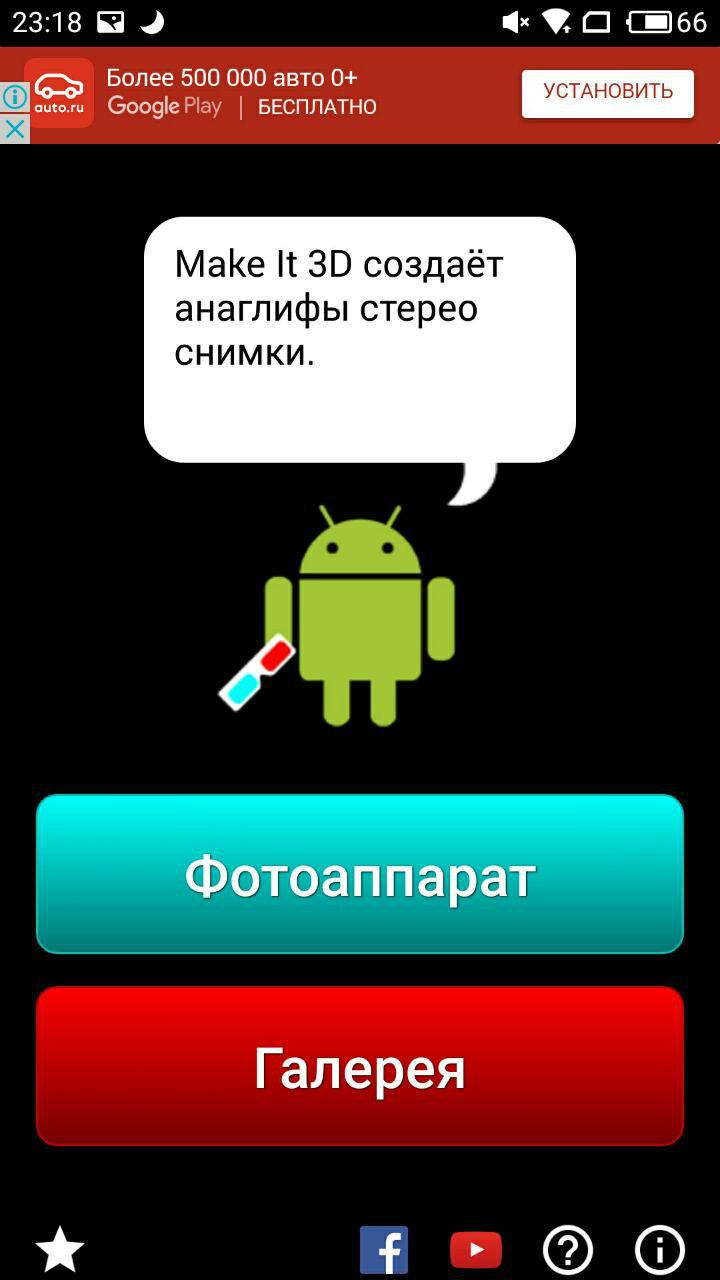
\includegraphics[width=0.45\linewidth]{pics/MakeIt1}
	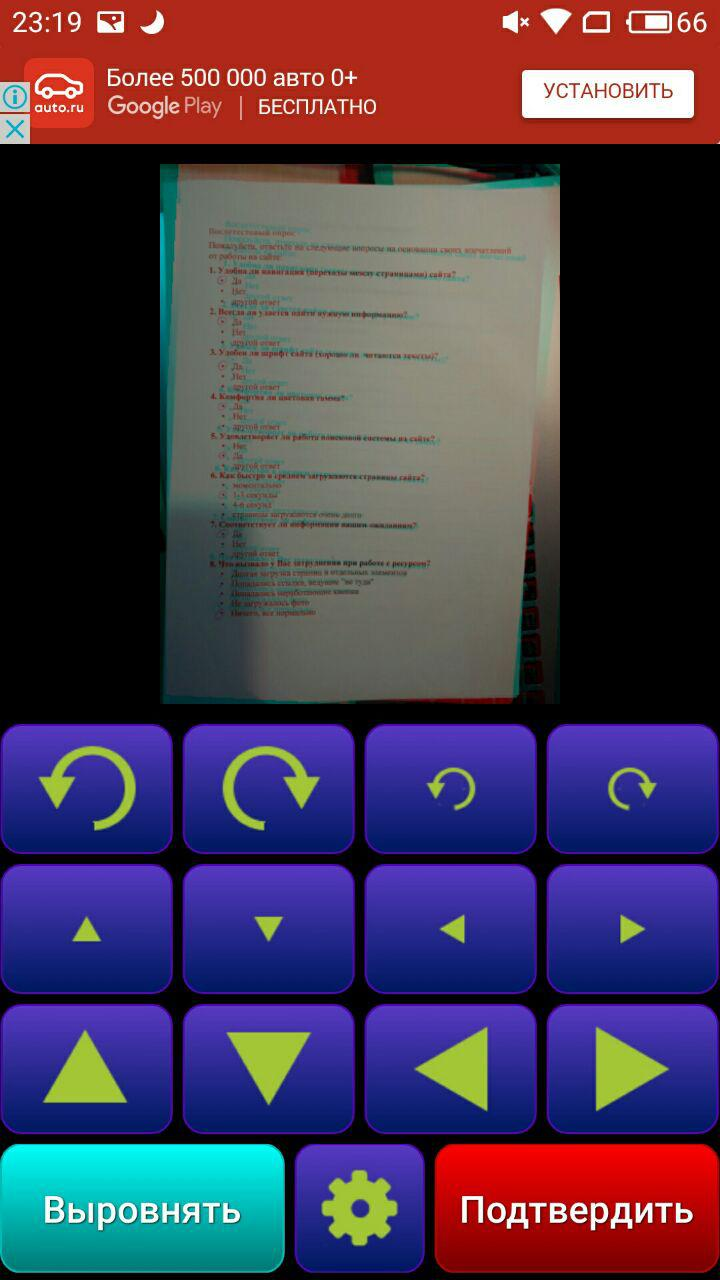
\includegraphics[width=0.45\linewidth]{pics/MakeIt2}
	\caption{MakeIt}
	\label{fig:MakeIt}
\end{figure}

\subsection{3D Effect}

Приложение, создающее анаглиф из одного изображения. Доступна возможность настройки степени смещение и выбор одного из трех вариантов смещения:  по горизонтали, по вертикали, по диагонали. Так предоставлена возможность выбора цвета стереоэффекта, например: красно-голубой, сине-желтый, зелёно-розовый. Изображение сохраняется в фотогалерею смартфона и выводит варианты «шэринга». (рисунок ~\ref{fig:3dEffect})

\begin{figure}[H]
	\centering
	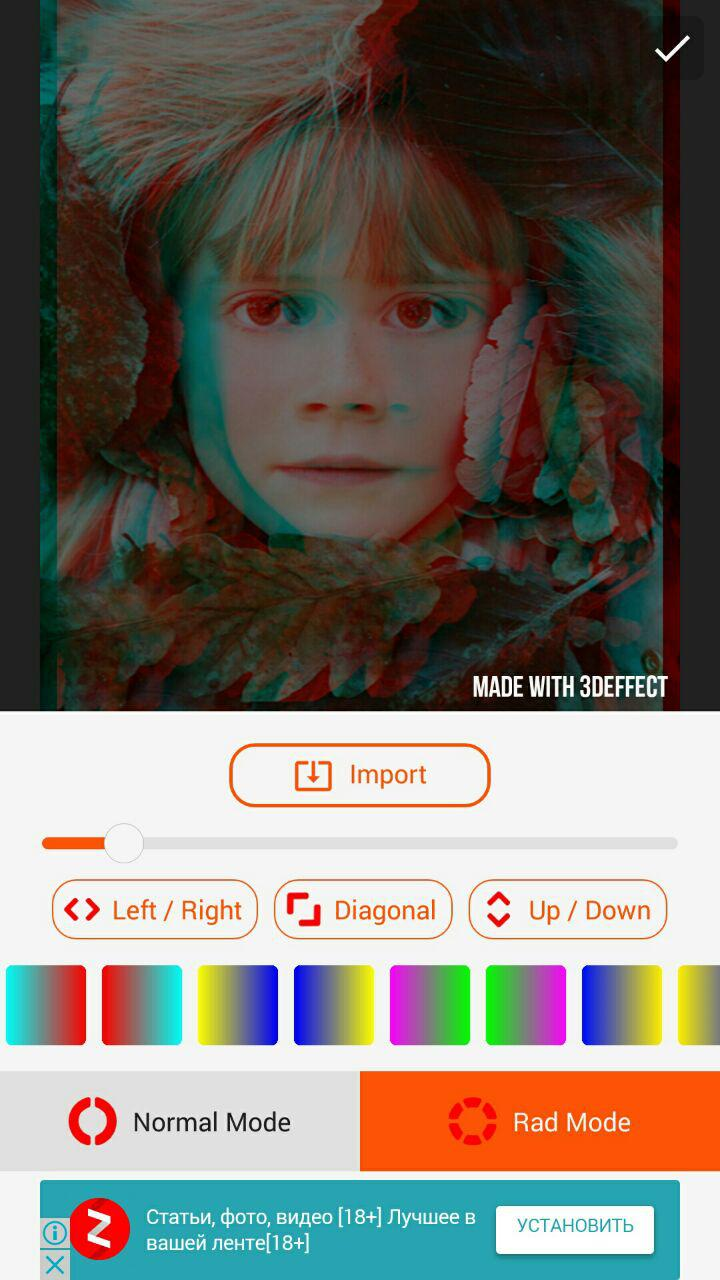
\includegraphics[width=0.45\linewidth]{pics/3dEffect1}
	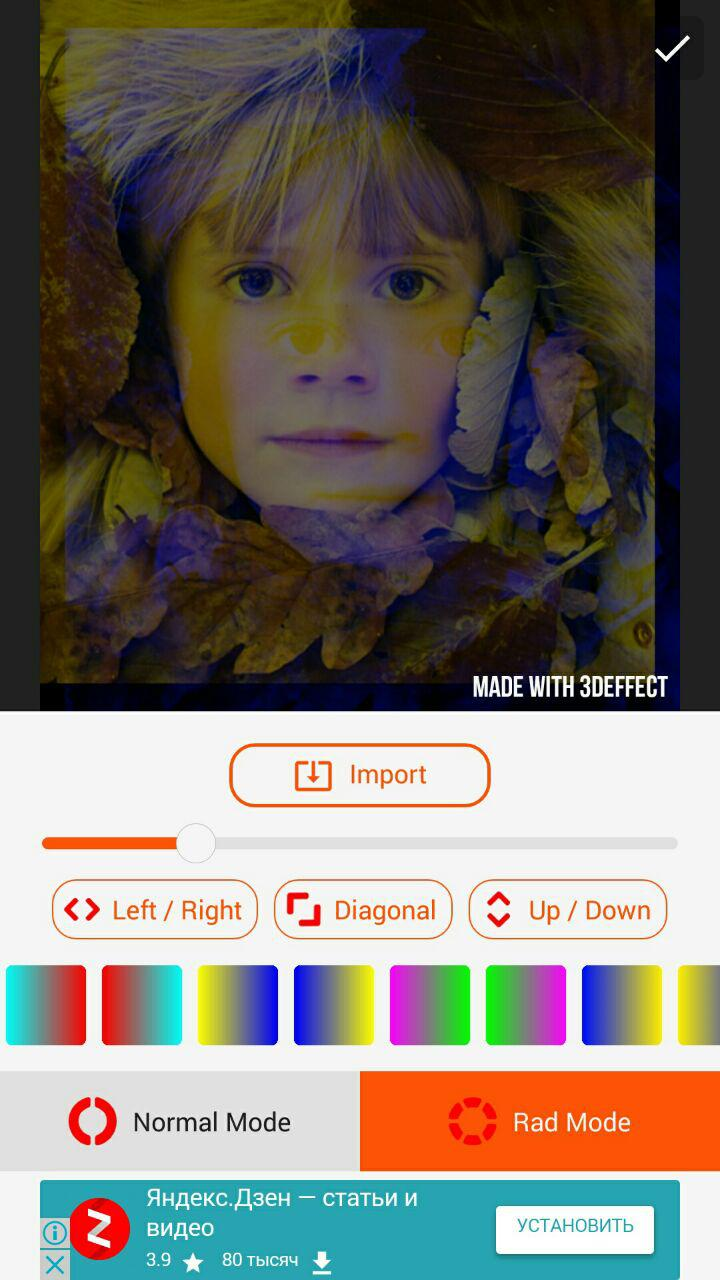
\includegraphics[width=0.45\linewidth]{pics/3dEffect2}
	\caption{3dEffect}
	\label{fig:3dEffect}
\end{figure}

\subsection{Motion Photo}

Инструмент, предоставляемый производителями смартфонов. Впервые появился в iOS 9 в 2015 году под названием Live Photos, а позже аналоги появились в Android-смартфонах, линейке Galaxy от Samsung, начиная с модели S7, а также в Google Pixel 2. Решение в корне отличается от варианта с созданием анаглифа, однако предоставляет возможность оживить фотографию, что так же является и результатом работы нашей разработки. Принцип работы заключается в постоянном сохранении в оперативную память устройства 1-3 секунд изображения с камеры, до момента нажатия на кнопку спуска затвора, после чего сохраняется еще один видеофрагмент. Таким образом, при просмотре обычного фото в галерее смартфона, появляется возможность увидеть живой момент съемки.

\subsection{Fyuse}

Fyuse совмещает в себе возможность создания пространственной фотографии и платформу для общения. По ходу использования приложение фокусируется на объекте, а затем при помощи графических подсказок на экране предлагает обойти объект камерой по орбите. Полученный результат представляет собой снимок, позволяющий перемещать камеру вида по орбите вокруг изображенного предмета при помощи свайпов или гироскопа смартфона. Фотографию можно сохранить или опубликовать прямо во Fyuse, являющейся так же и социальной сетью. (рисунок ~\ref{fig:Fyuse})

\begin{figure}[H]
	\centering
	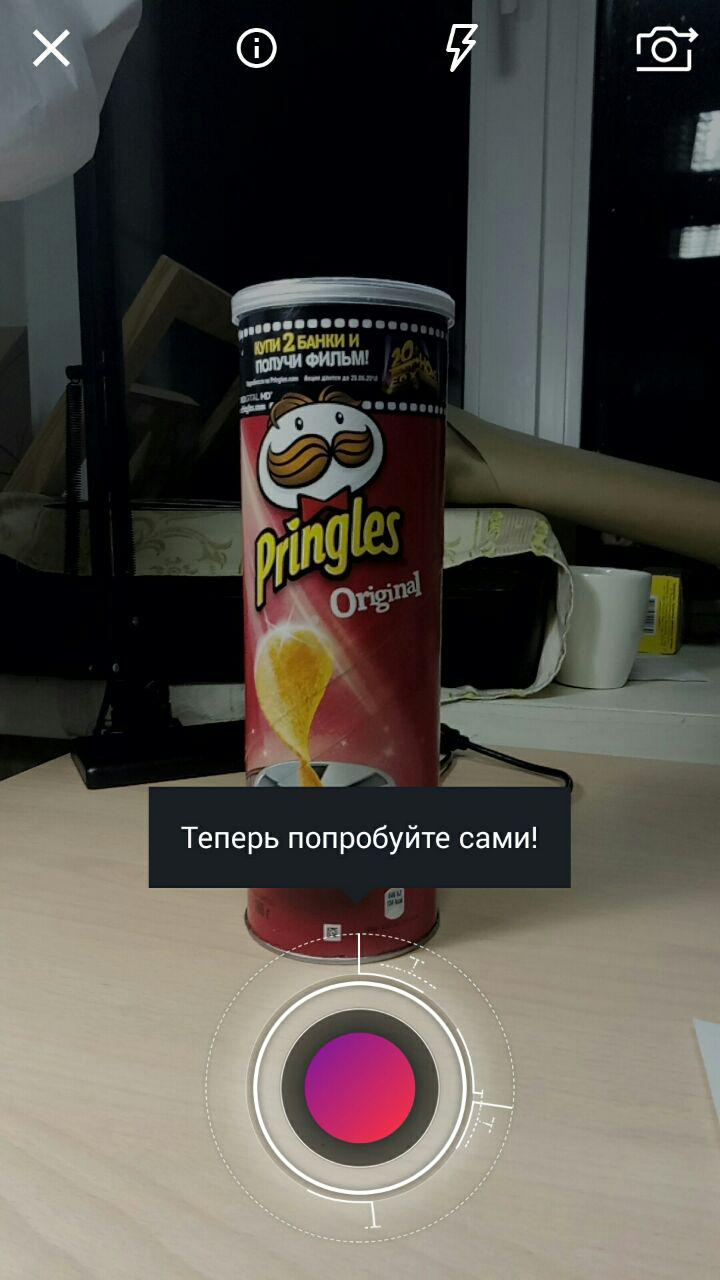
\includegraphics[width=0.45\linewidth]{pics/Fyuse1}
	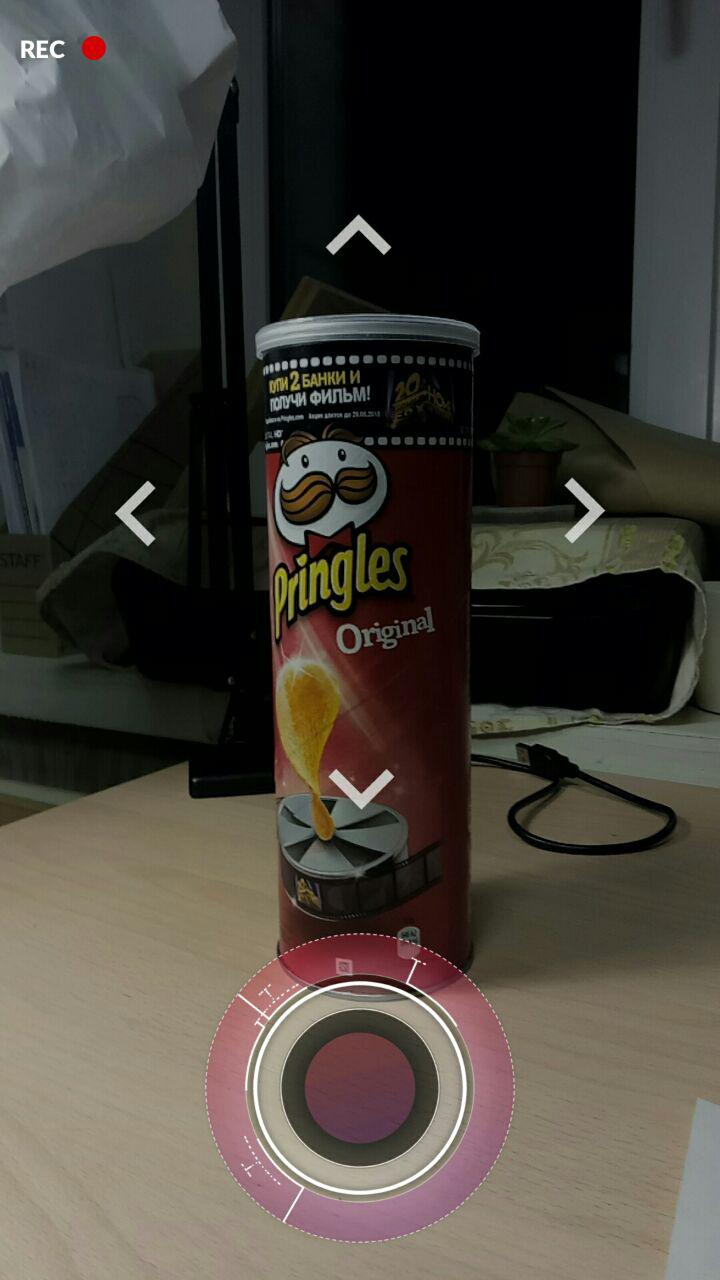
\includegraphics[width=0.45\linewidth]{pics/Fyuse2}
	\caption{Fyuse}
	\label{fig:Fyuse}
\end{figure}

\subsection{Вывод}
По результатам анализа существующих аналогов можно сделать вывод, что разработчики предлагают абсолютно разные способы оживления снимков. Для некоторых требуются определенный манипуляции еще при съемке, некоторые могут работать с готовыми фотографиями. Каждое решение по-своему уникально и интересно. Мы же предлагаем еще одно решение, особенностью которого является «оживление» уже готового снимка.


\section{Разработка пользовательского интерфейса мобильного приложения (UI/UX)}

Одна из важнейших задач в ходе создания мобильного приложения, преобразовывающего 2D снимки в объемные (3D) - разработка удобного и интуитивно-понятного пользовательского интерфейса. UI/UX (user Interface, user experience) составляющая, она же пользовательский интерфейс и пользовательский опыт, является более чем просто значимым элементом современного мобильного приложения. Удобство расположения элементов управления и приятное визуальное оформление напрямую влияют на настроение пользователя при использовании продукты. Именно некачественный UI/UX-дизайн отпугивает людей от использования многих приложений в пользу их более достойных альтернатив.

\subsection{Анализ интерфейсов смежных приложений}

Для использования в качестве референсов были подобраны приложения, принадлежащие широкому понятию «Приложения для работы с фото», так как узкоспециализированные решения не представляют интерфейса должного качества и удобства.

В список приложений для анализа попали такие приложения, как:  Prisma, Vinci, Snapster и Pixlr.

В первую очередь, целью сравнения являлся анализ особенностей пользовательского интерфейса этих приложений. Это обусловлено тем, что предполагаемая схема  взаимодействия пользователя с разрабатываемым приложением во много схожа с таковой в этих приложениях, за исключением некоторых их особенностей. Важные элементы для сравнения  - сценарий создания снимка с использованием фотокамеры смартфона и выбор снимка из галереи для дальнейшей отправки фотографии на обработку алгоритмом, преобразующим ее в 3D фотографию.

\subsubsection{Prisma}

Проанализировав пользовательский интерфейс первого приложения, Prisma (рисунок~\ref{fig:prisma}), можно заметить не очень удобное расположение элементов. Так, кнопка настроек, далеко не самая востребованная на фоне остальных, расположена в правом нижнем углу, куда доступ наиболее прост в условиях больших размеров современных смартфонов. В том время как кнопка смена камеры расположена в правом верхнем углу, куда доступ затруднительнее. Стоит отметить и факт смещения нижних иконок в углу экрана, что далеко не положительном образом сказывается на опыте использования приложения.

Также Prisma, в связи со своими социальными особенностями функционала, имеет навигационный бар в верхней части экрана, представленный фиксированными вкладками (fixed tabs), оформленным в соответствии с гайдлайнами material-дизайна (Material Design Guidelines), разработанными Google. В целом приложение лишь частично следует гайдлайнам от Google, что заметно на примере применения material-иконок и одновременно неверном использовании фаба (float action button).

Экран шейринга фотографии выполнен по примеру Instagram, с подобным размещением элементов и учетом особенностей Prisma.

\begin{figure}[H]
	\centering
	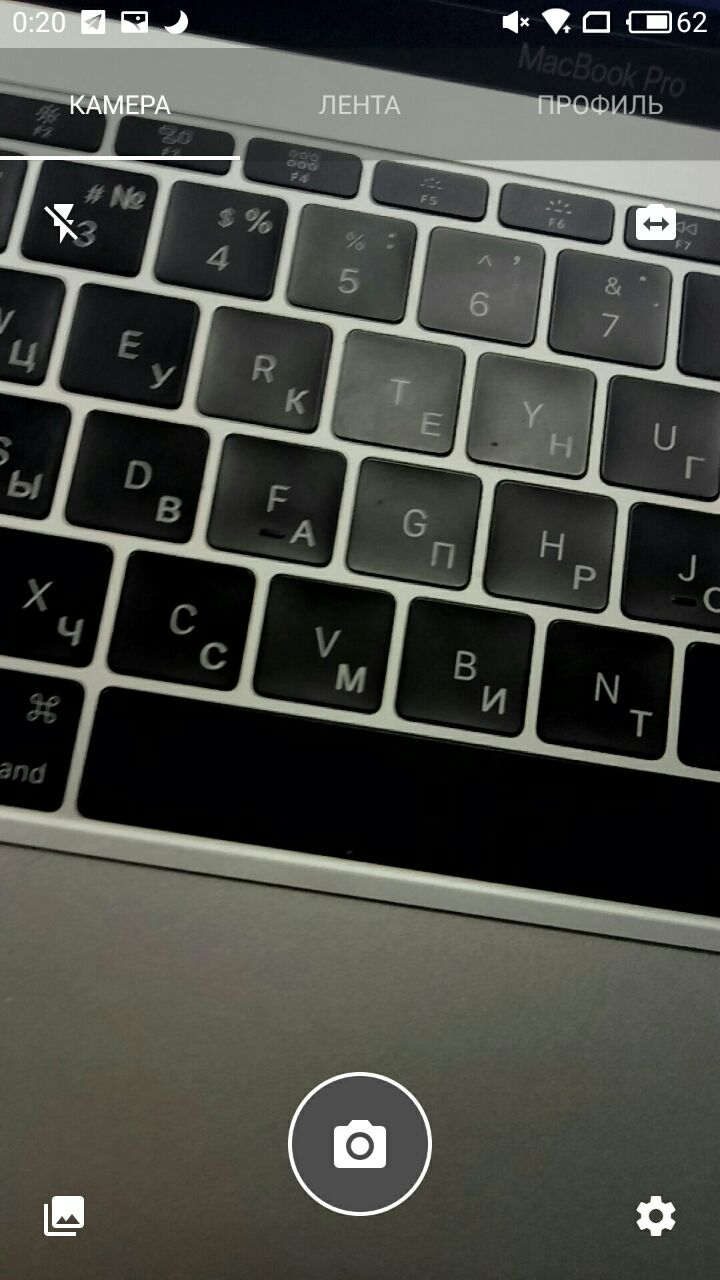
\includegraphics[width=0.45\linewidth]{pics/prisma1}
	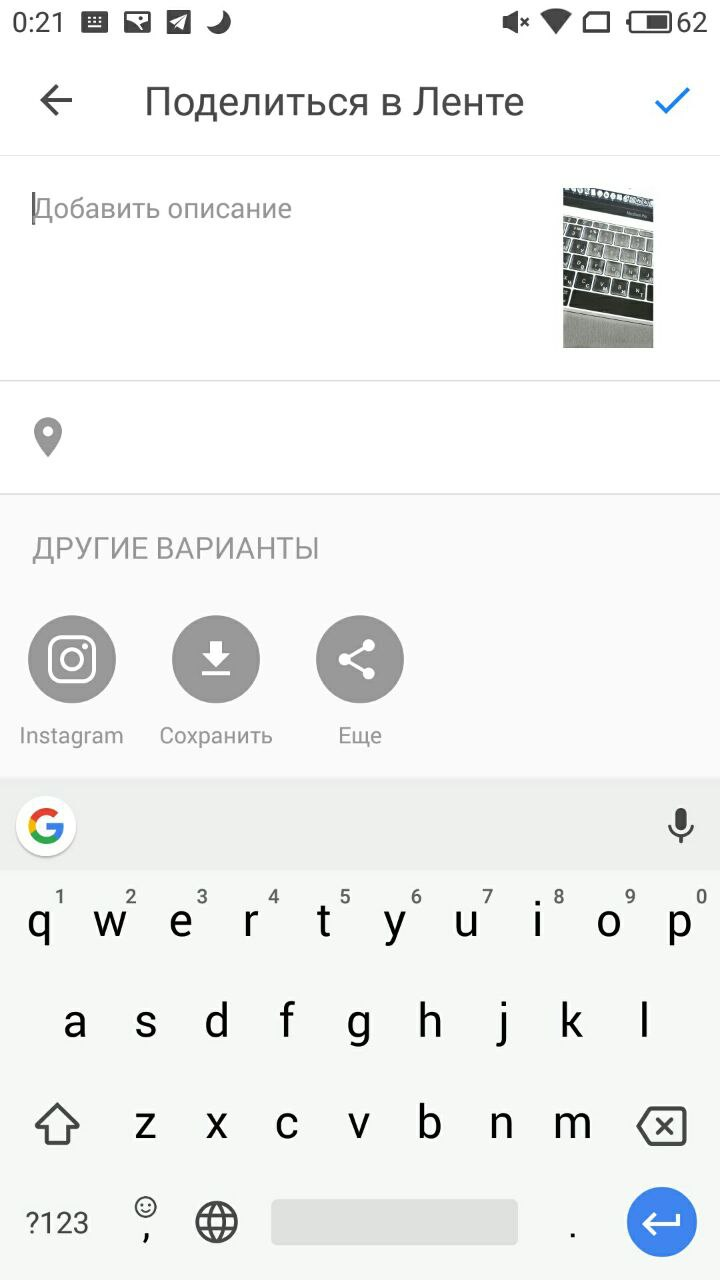
\includegraphics[width=0.45\linewidth]{pics/prisma2}
	\caption{Prisma}
	\label{fig:prisma}
\end{figure}

\subsubsection{Vinci}

Интерфейс Vinci (рисунок~\ref{fig:vinci}) выглядит более удачным, на фоне Prisma, и, забегая вперед, на фоне остальных выбранных приложений также, за исключением  Snapster. В нижней части удачно разместилась  выдвигающаяся панель с последними снимками, выше кнопка спуска затвора, включения вспышки и смены камеры. В верхнем углу разместилась иконка настроек. Такое разделение экрана обусловлено популярным соотношением сторон для снимков 4:3.

Плашка шейринга, появляющаяся в нижней части экрана, также весьма удобна для использования.

\begin{figure}[H]
	\centering
	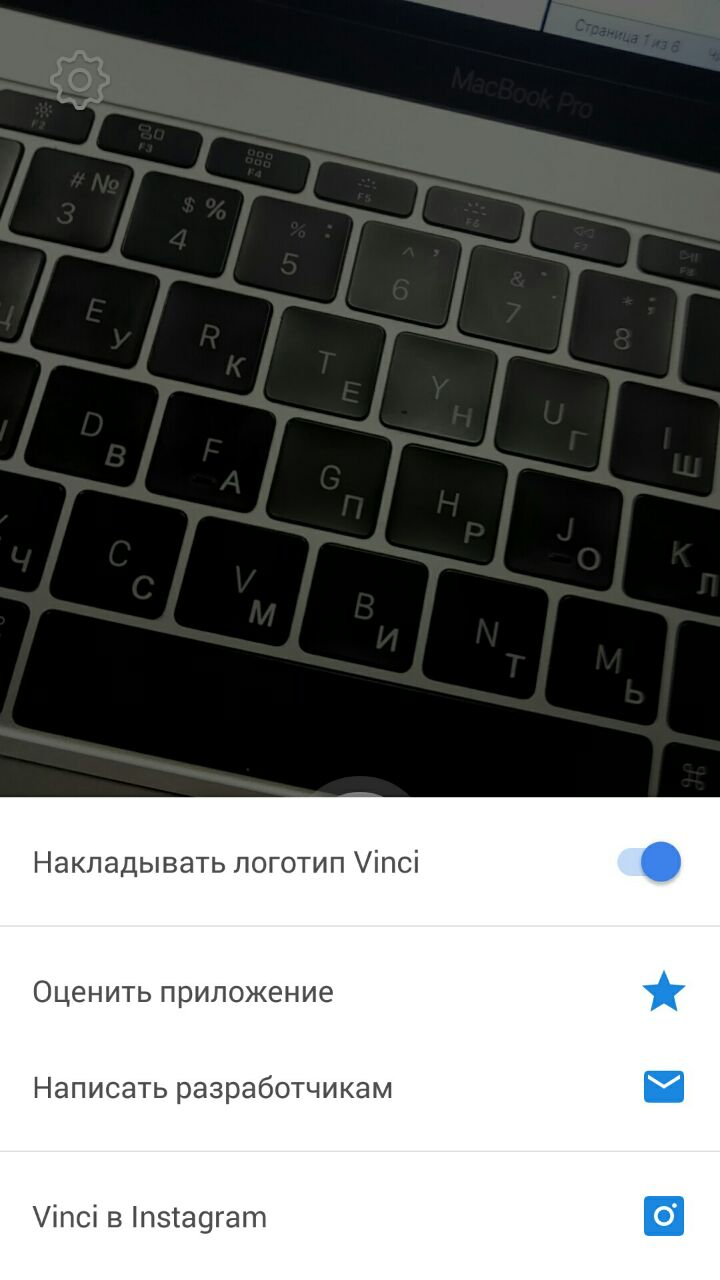
\includegraphics[width=0.3\linewidth]{pics/vinci1}
	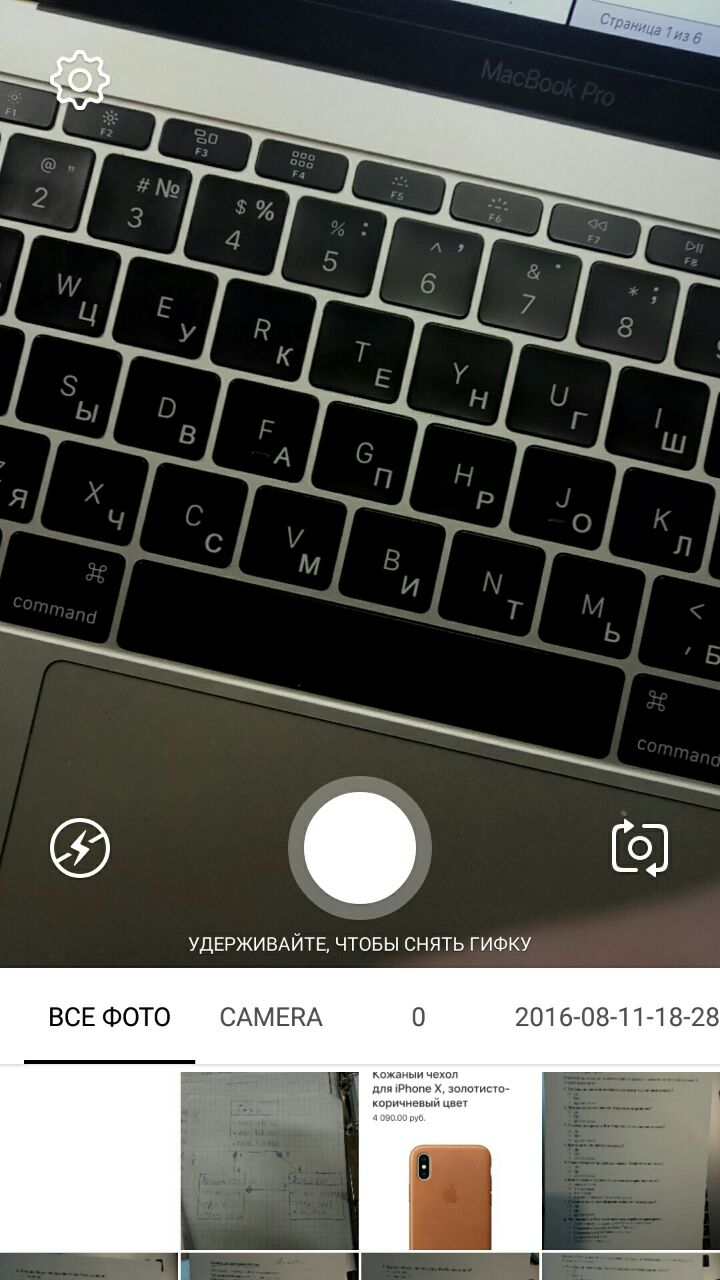
\includegraphics[width=0.3\linewidth]{pics/vinci2}
	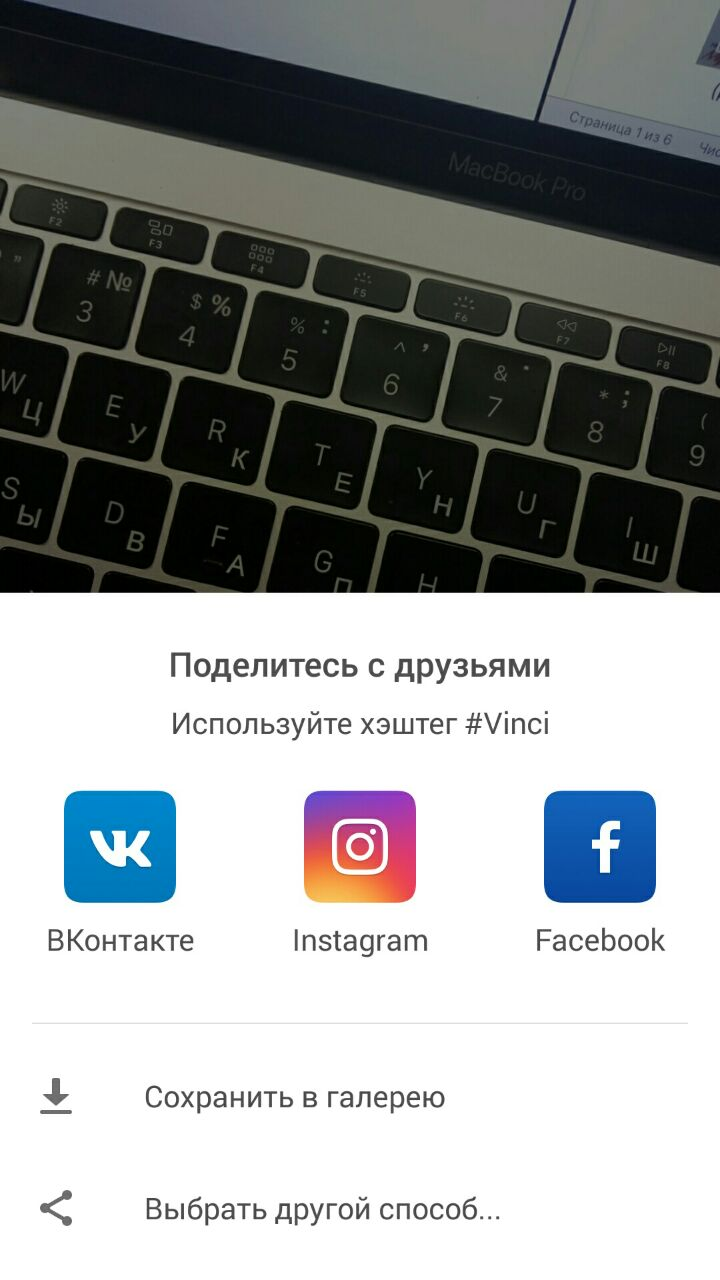
\includegraphics[width=0.3\linewidth]{pics/vinci3}
	\caption{Vinci}
	\label{fig:vinci}
\end{figure}

\subsubsection{Pixlr}

Особенностью интерфейса Pixlr (рисунок~\ref{fig:pixlr}),  в отличие от подобранных примеров, является присутствие стартового экрана, который, однако, несколько замедляет взаимодействие с приложением. Кнопки управление на экране камеры визуально неприятны и имеют непривычное соотношение размеров.

\begin{figure}[H]
	\centering
	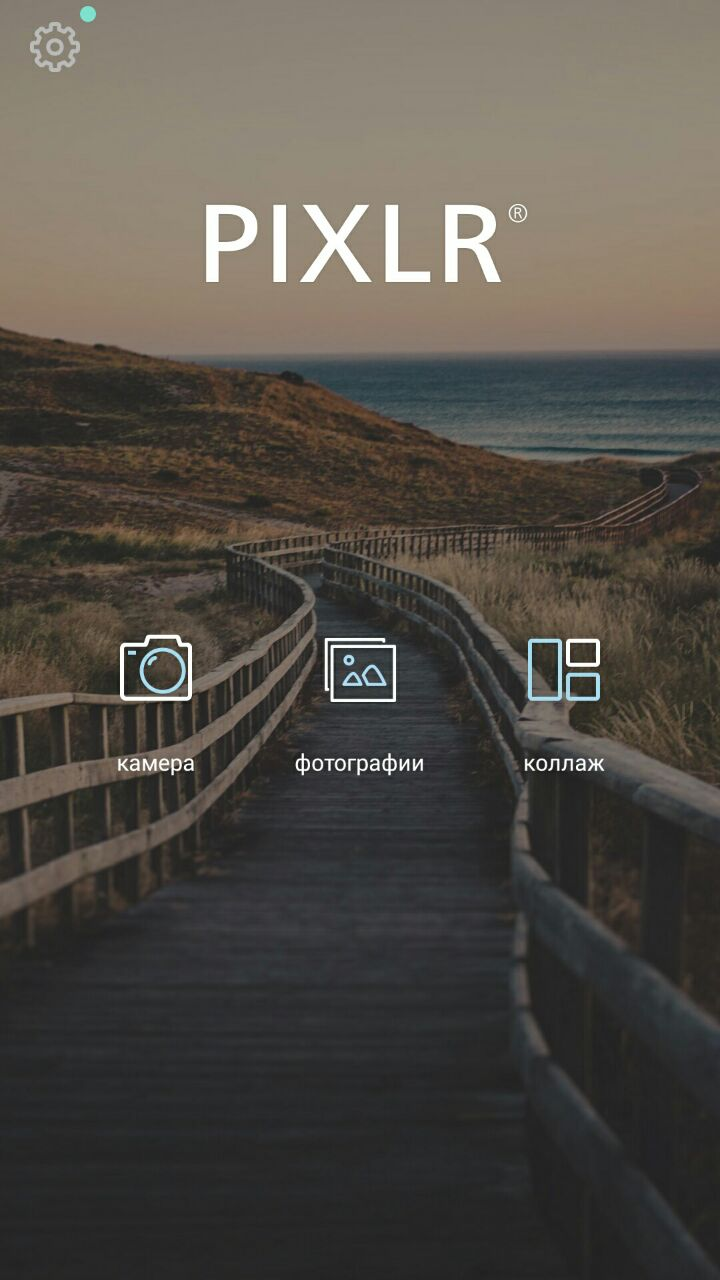
\includegraphics[width=0.45\linewidth]{pics/pixlr1}
	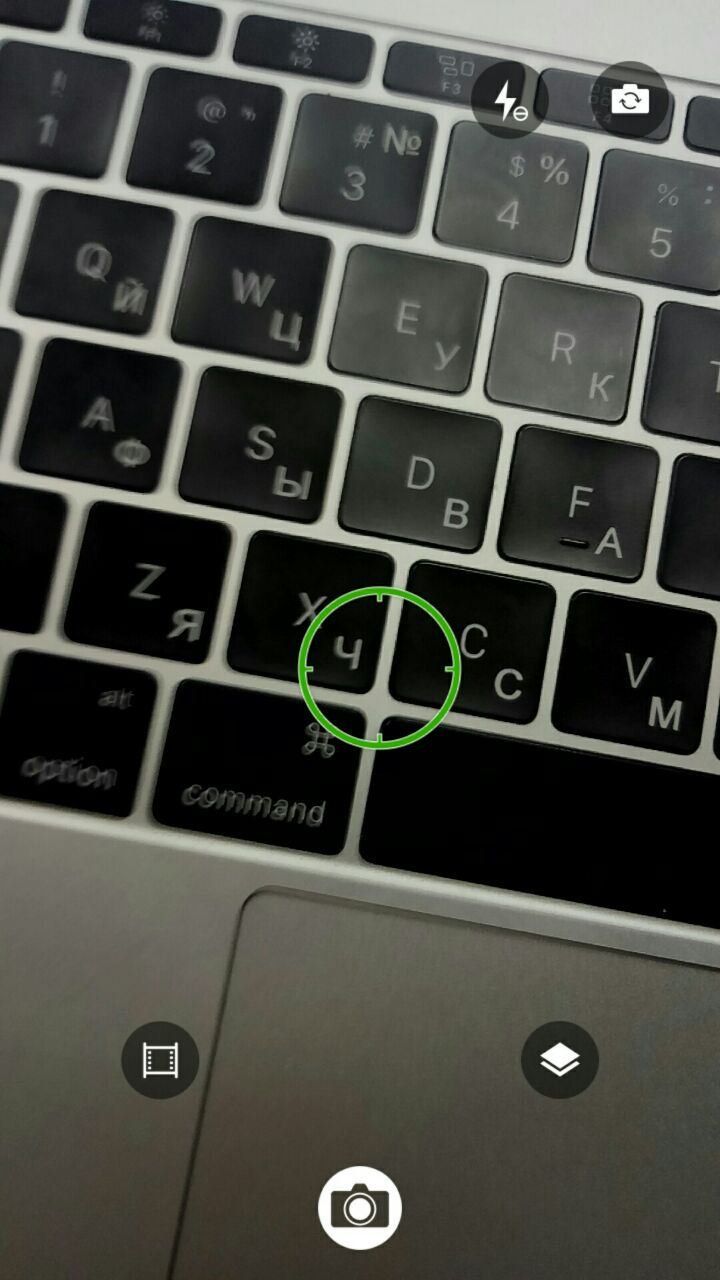
\includegraphics[width=0.45\linewidth]{pics/pixlr2}
	\caption{Pixlr}
	\label{fig:pixlr}
\end{figure}

\subsubsection{Snapster}

Как уже было сказано, Vinci и Snapster (рисунок~\ref{fig:snapster}) имеют примерно одинаковый уровень юзабилити, что объясняется одним и тем же авторством. В нижней части экрана размещен блок с последними снимками, но уже другим способ навигации - горизонтальной прокруткой (скроллом). Разработчик решил не внедрять кнопку настроек, нашлось место для полезно кнопки активации сетки. В целом, приложение Snapster, являясь экспериментальным проектом социальной сети VK, претерпело за время своего существования довольно сильные изменения. Если в первоначальном виде приложение дублировало основной функционал модуля «Фотографии» из социальной сети VK и расширяло его возможности, то сейчас, не сыскав популярности, было урезано до простенького фоторедактора.

\begin{figure}[H]
	\centering
	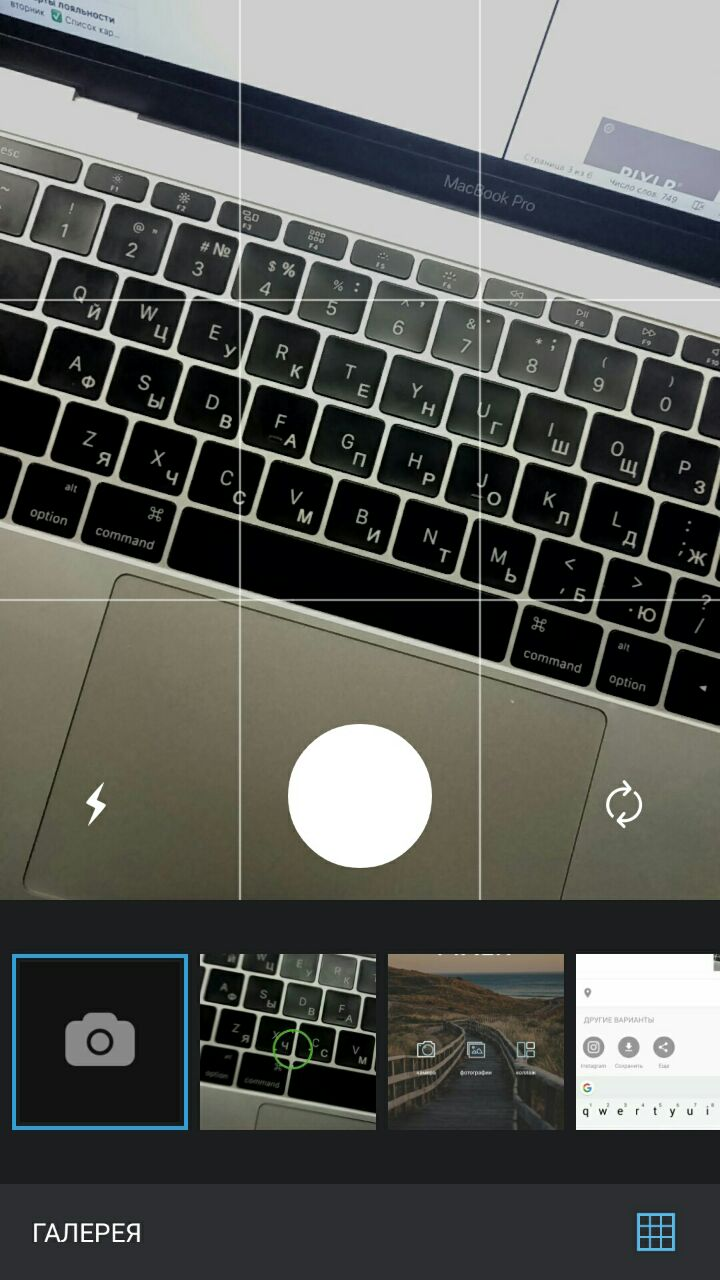
\includegraphics[width=0.45\linewidth]{pics/snapster1}
	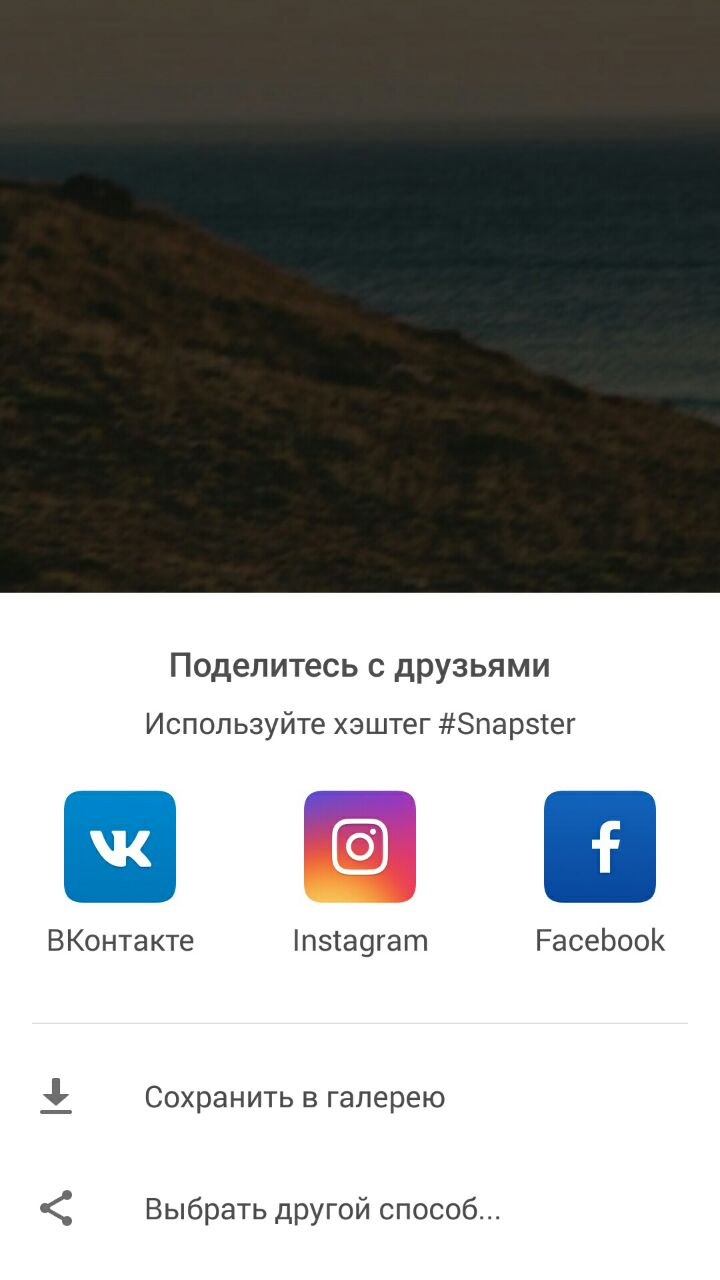
\includegraphics[width=0.45\linewidth]{pics/snapster2}
	\caption{Snapster}
	\label{fig:snapster}
\end{figure}

\subsection{Разработка пользовательского интерфейса мобильного приложения (UI/UX)}

Интерфейс Android-смартфона мобильного приложения для преобразования 2D фотографии в 3D вид выполнен в соответствии с гайдлайнами Material Design. Отступы, иконки и используемые шрифты полностью соответствуют руководству от Google~\cite{google}. 

Расположение элементов управление выполнено с учетом лучших особенностей приложений-аналогов.

На главный экран камеры (рисунок~\ref{fig:Artboard}) выведены следующие функции:

\begin{itemize}
	\item Спуск затвора;
	\item Выбор фото из галереи;
	\item Смена камеры;
	\item Управление вспышкой;
	\item Переход к настройкам и справке.
\end{itemize}

\begin{figure}[H]
	\centering
	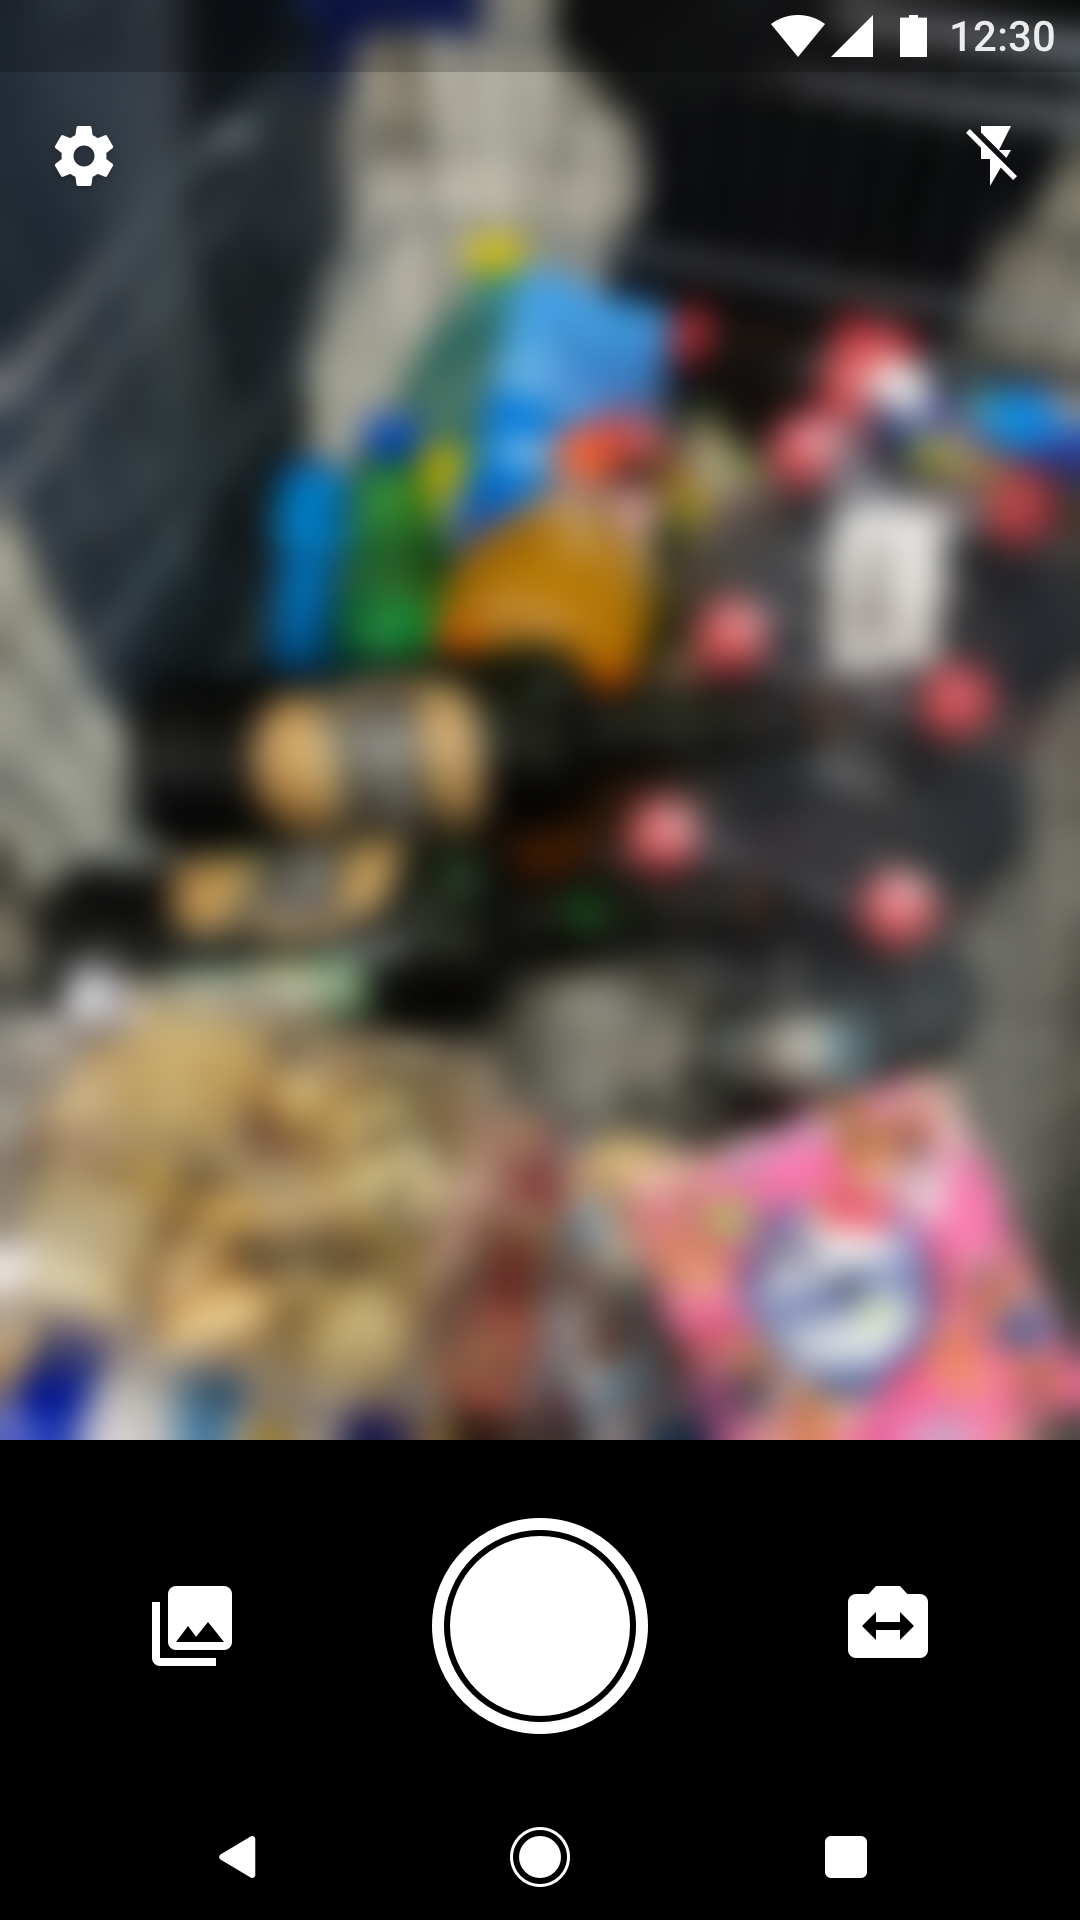
\includegraphics[width=0.6\linewidth]{pics/Artboard}
	\caption{Окно с камерой}
	\label{fig:Artboard}
\end{figure}

На экране с обработанной фотографией по нажатии кнопки «Далее» появляется bottom sheet (рисунок~\ref{fig:Artboard2}), включающий в себя быстрые функции шеринга и сохранения полученного фото в галерею.

\begin{figure}[H]
	\centering
	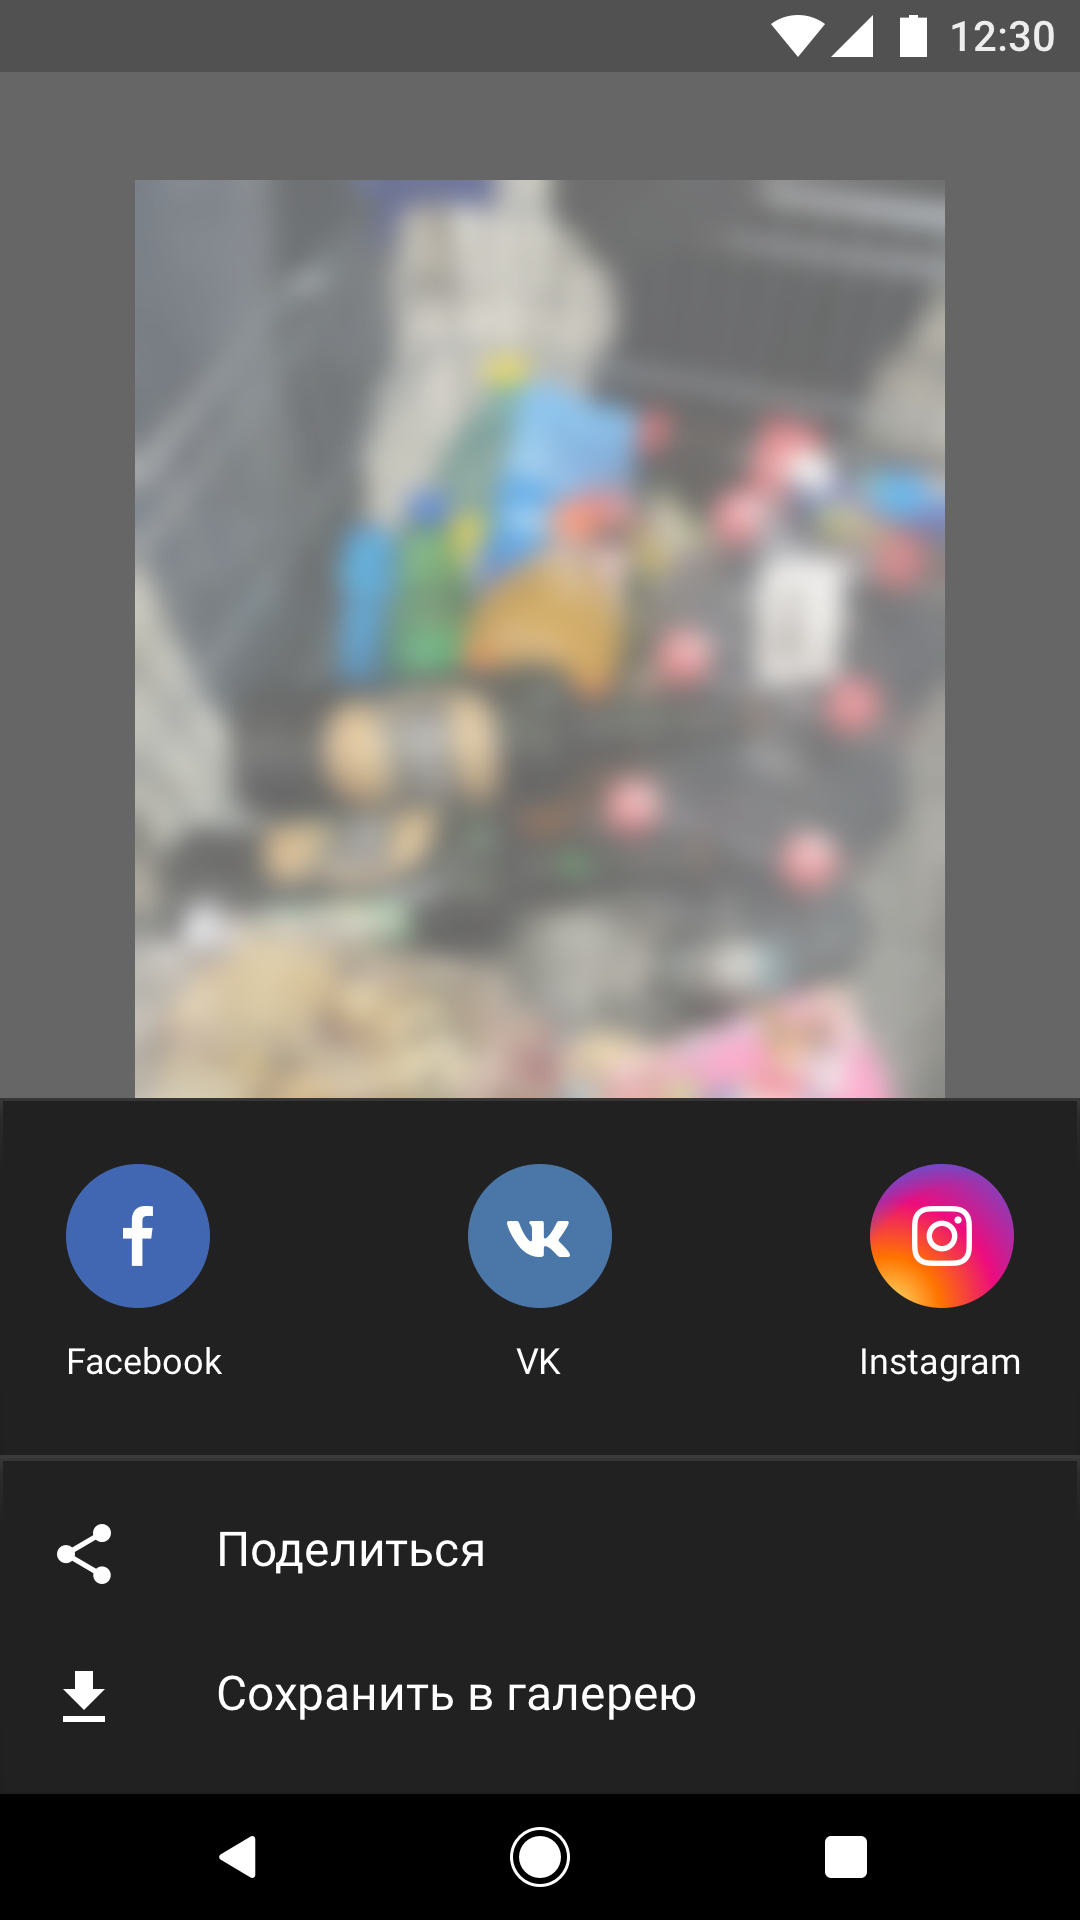
\includegraphics[width=0.6\linewidth]{pics/Artboard2}
	\caption{Окно с просмотром фото}
	\label{fig:Artboard2}
\end{figure}

При создании пользовательского интерфейса приложения были проанализированы современные, с аналогичным функционалом мобильные приложения в целом. Был сделан акцент на необходимости создания современного, функционального и не перегруженного пользовательского интерфейса. В результате проведенного анализа был создан пользовательский интерфейс мобильного приложения для преобразования 2D фотографий в 3D вид.


\subsection{Проектирование структуры приложения}

Одна из важнейших задач в ходе создания мобильного приложения, преобразовывающего 2D снимки в объемные (3D) - разработка удобного и интуитивно-понятного пользовательского интерфейса. UI/UX (user Interface, user experience) составляющая, она же пользовательский интерфейс и пользовательский опыт, является более чем просто значимым элементом современного мобильного приложения. Удобство расположения элементов управления и приятное визуальное оформление напрямую влияют на настроение пользователя при использовании продукты. Именно некачественный UI/UX-дизайн отпугивает людей от использования многих приложений в пользу их более достойных альтернатив.

На главный экран камеры (рисунок~\ref{fig:Artboard}) выведены следующие функции:

\begin{itemize}
	\item Спуск затвора;
	\item Выбор фото из галереи;
	\item Смена камеры;
	\item Управление вспышкой;
	\item Переход к настройкам и справке.
\end{itemize}

\begin{figure}[H]
	\centering
	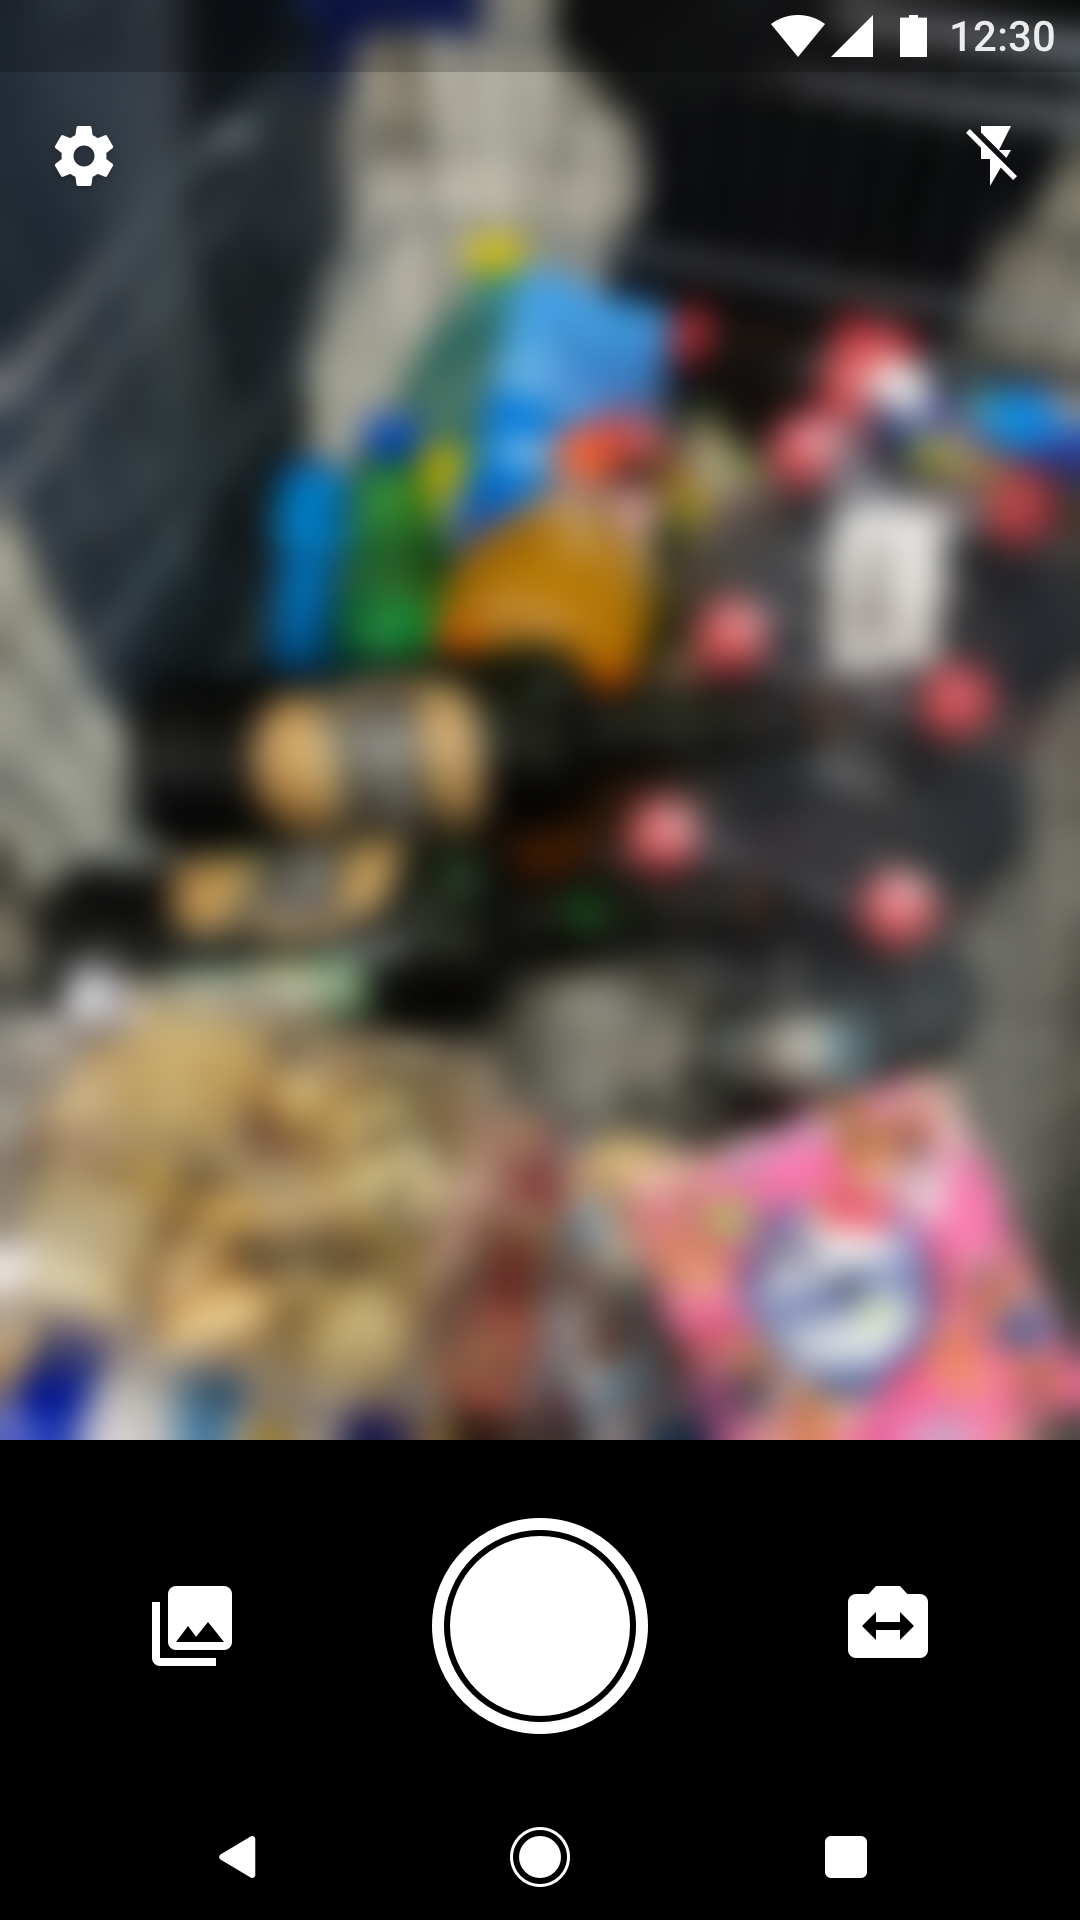
\includegraphics[width=0.6\linewidth]{pics/Artboard}
	\caption{Окно с камерой}
	\label{fig:Artboard}
\end{figure}

На экране с обработанной фотографией по нажатии кнопки «Далее» появляется bottom sheet (рисунок~\ref{fig:Artboard2}), включающий в себя быстрые функции шеринга и сохранения полученного фото в галерею.

\begin{figure}[H]
	\centering
	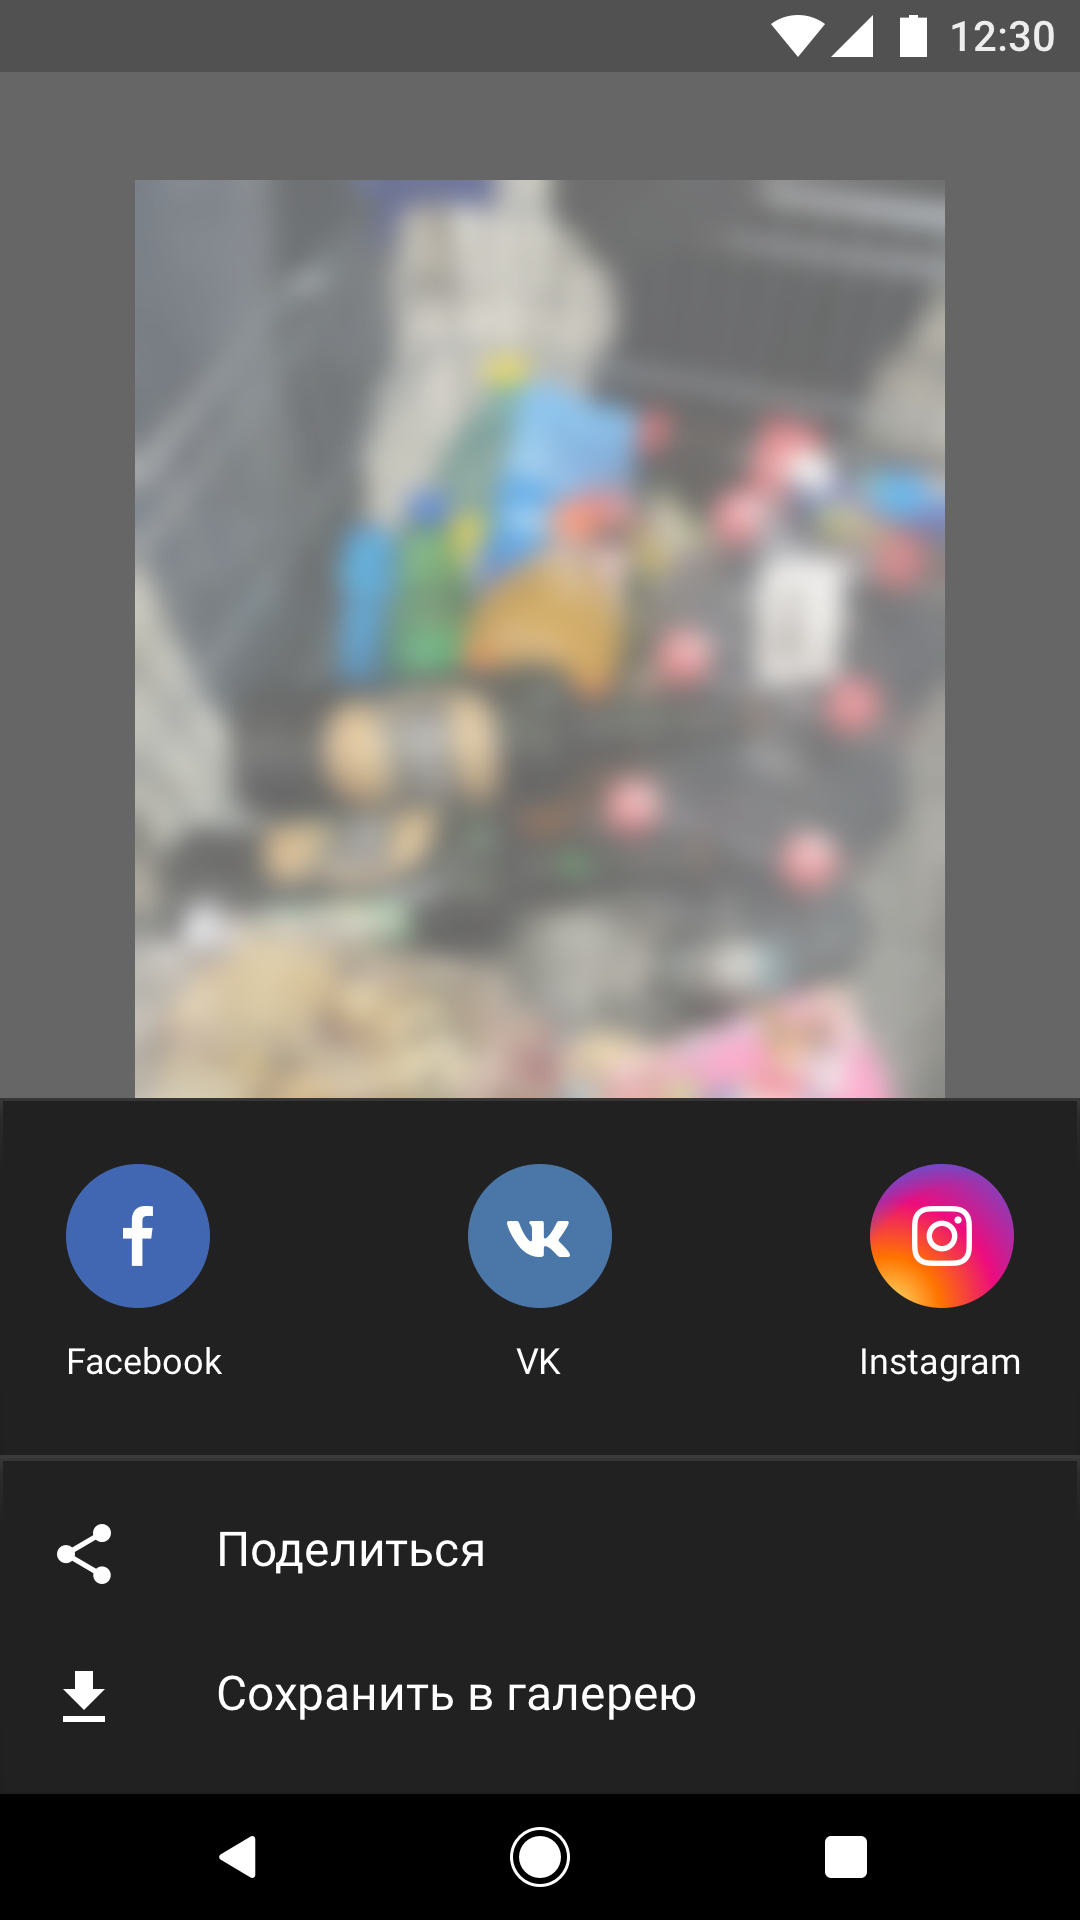
\includegraphics[width=0.6\linewidth]{pics/Artboard2}
	\caption{Окно с просмотром фото}
	\label{fig:Artboard2}
\end{figure}

При создании пользовательского интерфейса приложения были проанализированы современные, с аналогичным функционалом мобильные приложения в целом. Был сделан акцент на необходимости создания современного, функционального и не перегруженного пользовательского интерфейса. В результате проведенного анализа был создан пользовательский интерфейс мобильного приложения для преобразования 2D фотографий в 3D вид.

\subsection{Разработка мобильного приложения}

Рассмотрю практичный пример, когда программно запускаю приложение "Камера", а полученную фотографию сохраняю в папке.~\cite{camera}

В манифесте нужно добавить разрешение на запись файла в хранилище и указать требование наличия камеры.

Используем статическую константу ACTION\_IMAGE\_CAPTURE из объекта MediaStore для создания намерения, которое потом нужно передать методу startActivityForResult(). Разместим на форме кнопку и ImageView, в который будем помещать полученный снимок. Полученное с камеры изображение можно обработать в методе onActivityResult()

При тестировании примера на своём телефоне я обнаружил небольшую проблему - когда снимок передавался обратно на моё приложение, то оно находилось в альбомном режиме, а потом возвращалось в портретный режим. При этом полученный снимок терялся. Поэтому перед нажатием кнопки я поворачивал телефон в альбомный режим, чтобы пример работал корректно. Поэтому надо предусмотреть подобное поведение, например, запретить приложению реагировать на поворот и таким образом избежать перезапуска Activity. 

По умолчанию фотография возвращается в виде объекта Bitmap, содержащего миниатюру. Этот объект находится в параметре data, передаваемом в метод onActivityResult(). Чтобы получить миниатюру в виде объекта Bitmap, нужно вызвать метод getParcelableExtra() из намерения, передав ему строковое значение data.

(рисунок~\ref{fig:my})

\begin{figure}[H]
	\centering
	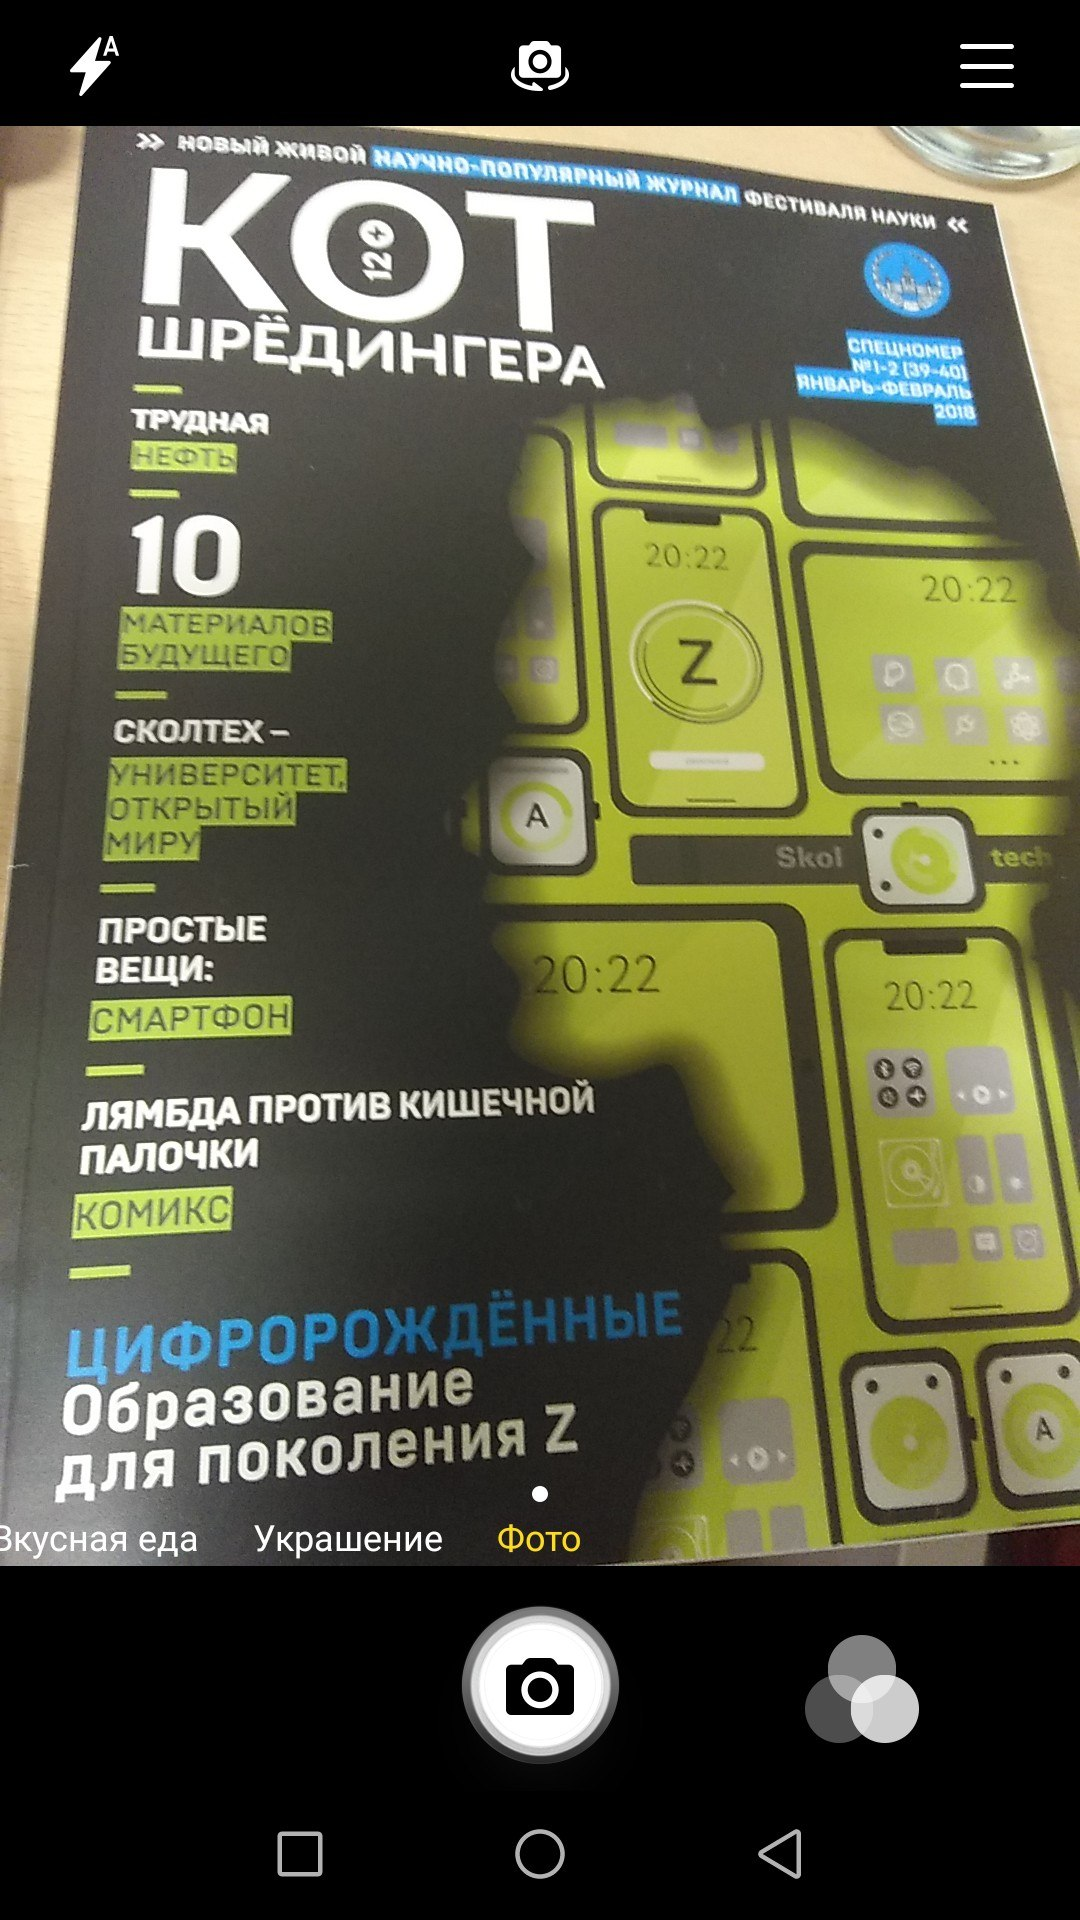
\includegraphics[width=0.4\linewidth]{pics/main}
	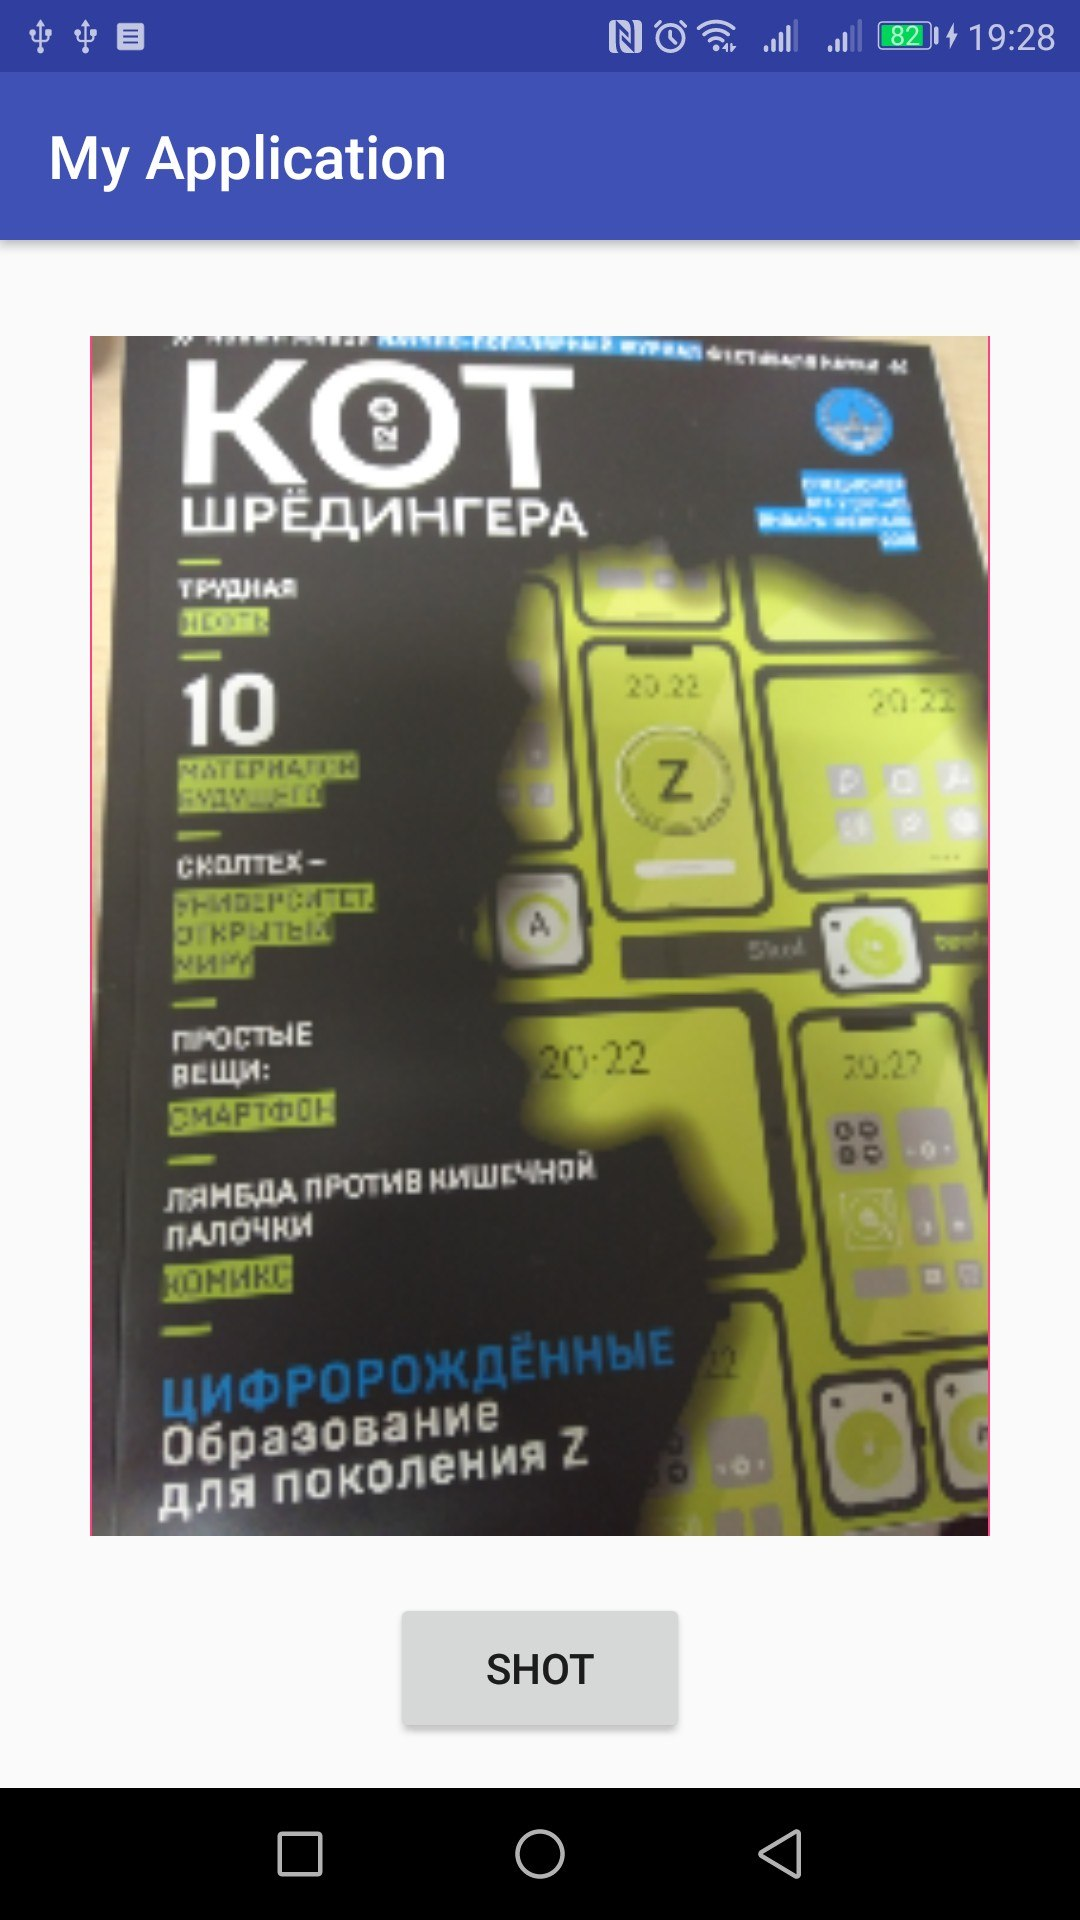
\includegraphics[width=0.4\linewidth]{pics/camera}
	\caption{Результат работы приложения}
	\label{fig:my}
\end{figure}